\documentclass[conference]{IEEEtran}
\usepackage{cite}
\usepackage{amsmath,amssymb,amsfonts}
\usepackage{graphicx}
\usepackage{url}

\graphicspath{{../docs/figures/}}

\begin{document}

\title{Supplement: How Much Can Conjunction Message Histories Predict Beyond Persistence?}

\author{\IEEEauthorblockN{Arjun Vijay Prakash}}
\maketitle

This supplement holds overflow tables and figures for the IEEE conference paper. Confirmatory claims remain in the main text. Code: \url{https://github.com/ArjunCodess/PRISM}.

\section{Hypothesis checklist}

\begin{itemize}
\item H1: matched-cohort $\Delta$MAE $4.49\to 0.03$ --- supported, with the 12~h CI covering zero.
\item H2: floor-excluded MAE worse than persistence at the primary split, and non-floor $\Delta$MAE negative at every matched horizon --- supported.
\item H3: ESA $L$, LOO 66/66, official test --- supported under this protocol.
\item H4a: $\log\det$ vs movement $\rho=0.399$ --- univariate yes; partial coefficient reverses after controlling for risk.
\item H4b: gap vs floor AUC 0.819 --- supported.
\item H4c: gap vs movement $\rho=-0.768$ --- supported (negative).
\end{itemize}

\section{Protocol}

Fig.~\ref{fig:protocol} is the leakage-safe pipeline. All model and policy choices were frozen before official-test evaluation.

\begin{figure}[t]
\centerline{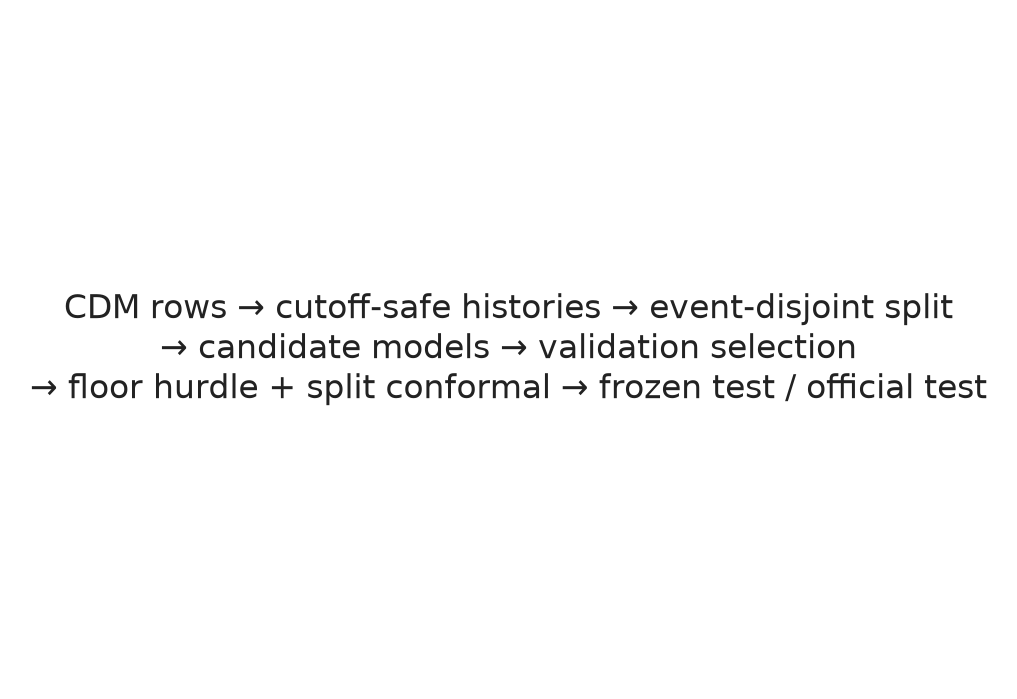
\includegraphics[width=\columnwidth]{protocol-flow.png}}
\caption{From cutoff-safe CDMs to a frozen test. Validation selects the floor hurdle; official-test scores are reports only.}
\label{fig:protocol}
\end{figure}

\section{Feature families}

The shipped feature table has 234 numeric columns: 77 snapshot (CDM fields plus derived geometry and object-type dummies), 68 history summaries, and 88 covariance trends. History stems are risk, miss distance, relative speed, max-risk estimate, and observation counts. Covariance stems are RTN sigmas and log position-covariance determinants. All rows have $\mathrm{time\_to\_tca}$ at or above the cutoff. $\texttt{dilution\_gap}$ is excluded from the shipped booster. The full name list is \texttt{ml/artifacts/feature\_schema.json}.

\section{Ablation}

\begin{figure}[t]
\centerline{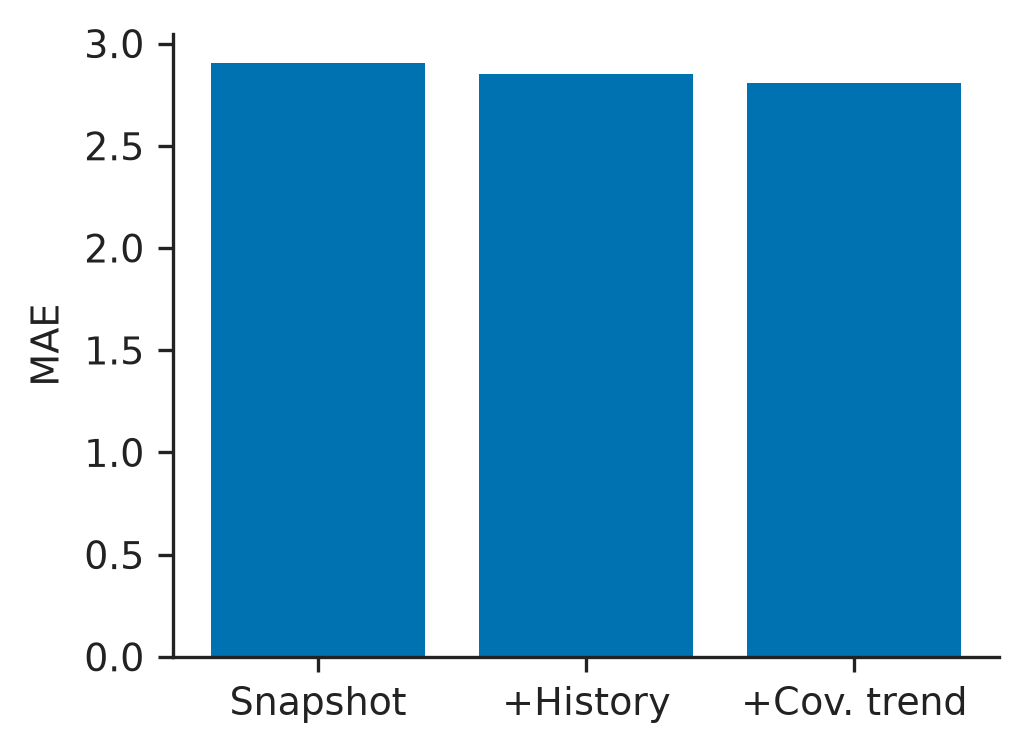
\includegraphics[width=\columnwidth]{feature-ablation-paper.png}}
\caption{Unguarded XGBoost MAE: snapshot, plus history, plus covariance trends.}
\label{fig:ablation}
\end{figure}

Snapshot MAE 2.904; after history 2.851; after covariance trends 2.808. History adds a small increment relative to the snapshot itself.

\section{Floor-classifier thresholds}

Thresholds 0.05 / 0.10 / 0.15 / 0.20 / 0.30 / 0.50 were scored on the frozen hurdle probabilities without retuning. The validation-selected operating point remains 0.15 (TP 1319, FP 174, FN 33, TN 133). False positives have median later $y=-14.3$ and mean snapshot risk $-14.9$.

\section{Five-seed redraws}

Seeds 42--46 retrain unguarded and residual XGBoost on grouped event splits. Unguarded MAE advantage $2.34\pm 0.04$; floor-excluded MAE $7.78\pm 0.21$; persistence floor-excluded $4.32\pm 0.23$. Seed 42 remains the reported row.

\section{Unmatched horizon table}

The overlapping-set table in earlier drafts mixed cohort change with horizon: advantages 4.534 / 2.272 / 0.524 / 0.060 at 72 / 48 / 24 / 12~h. The matched-cohort table in the main paper is the H1 result.

\section{Gap quartiles}

Train-quartile edges of $\texttt{max\_risk\_estimate}-\texttt{risk}$ on the frozen test: Q1 floor rate 0.556 and mean $|y-\mathrm{risk}|=13.03$; Q3--Q4 floor rates above 0.95 and mean movement below 0.75.

\section{Residual SHAP}

\begin{figure}[t]
\centerline{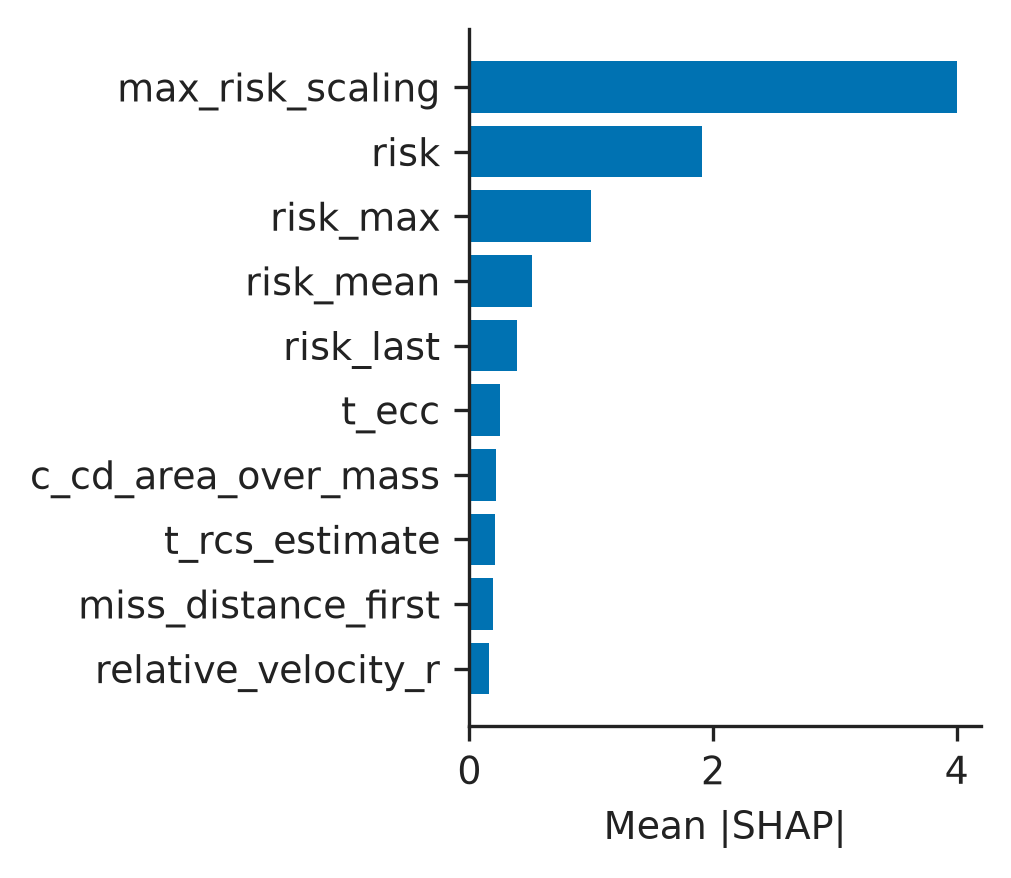
\includegraphics[width=\columnwidth]{residual-shap.png}}
\caption{Mean $|$SHAP$|$ of the residual regressor on 80 test rows. Risk-trajectory fields dominate; this is not a physical cause.}
\label{fig:shap}
\end{figure}

\section{Reproducibility checklist}

\begin{itemize}
\item Code: \url{https://github.com/ArjunCodess/PRISM}
\item Dataset: ESA Kelvins training archive and Zenodo 4463683
\item Split seed 42; IDs in \texttt{ml/artifacts/split\_manifest.json}
\item XGBoost: 250 trees, depth 4, learning rate 0.05, subsample 0.85, colsample 0.8, min-child-weight 6, $\ell_1=0.1$, $\ell_2=2.0$, no early stopping, native NaN
\item Floor classifier: 180 trees, depth 3, threshold 0.15, no persist guard
\item Figures: \texttt{python ml/src/plots.py}
\item Official test frozen before look; no retune
\end{itemize}

\end{document}
